\section{Galilean Relativity}

\subsection{Spacetime Diagrams}

Remind that Gelilean relativity states that the laws of motion are the same in all inertial reference frames.\\
We discussed before that, observers in different reference frames will agree on certain things, like the time and space (or space/time, $\Delta x$), the mass and indeed the laws of motion, but
they will disagree on other quantities like the velocity, momentum, kinetic energy, and even the position of physical objects.\\

The most important quantity is actually the position of an object $x$, and to understand how observers disagree on positions, we'll be 
studying spacetime diagrams.
A spacetime diagram is a tool for visualizing the motion of objects in different frames of reference.\\

A specetime diagram has the time $t$ on the vertical axis, increasing towards north, and the position $x$ as horizontal axis, increasing towards the right.
Let's first try to visualize an object standing still, starting at the origin at position $x = 0$.\\
As time passes, if the object stays still, no movement is done on its position, so the movement is simply a straight vertical line. It's traveling
through time but not through space. The path followed is called world-line. \\

Another example is an object moving at a constant speed of $25 m/s$ to the right. If this starts at the origin, after 1 second, 
it will have traveled $25 m$ to the right, after 2 seconds, its position will be $50 m$ to the right and so on.\\
Its world-line is a diagonal line pointint to the upper right.\\

The fastest the speed, the closer the world-line is to the horizontal axis. The slower, the closer to the vertical.\\

\textbf{Now, a really important point}, remember that in Galilean relativity, all motion is relative to something else, and that there's no
special reference frame that's at rest. Let's take a person, stationary, with a world-line moving only vertically through time, and a car, moving 
also through space at a constant speed.\\
From the point of view of the person, he's stationary, and the car is moving to the right. But from the point of view of the moving car, it's stationary, and the person is moving
to the left, along with the road and the entire neighborhood.
So, if we draw on the spacetime diagram, the person world-line as vertical, and the car moving world-line as diagonally pointing to the upper right, we're
drawing the spacetime diagram from the point of view of the person.\\
But it would equally correct drawing the spacetime diagram from the car's point of view, where the car is stationary, and the person is diagonally moving to the upper left.
Even though the two spacetime diagrams look different, they actually describe the exact same situation and the same physics, just from different points of view.\\

\textbf{We can always re-arrange a spacetime diagram, so that any object of our choice is stationary (i.e. representing the physics from the point of view of the object).
In order to do so, we have to re-arrange the time "slices" to make that object world-line vertical.
There's no special stationary frame of reference, and we can always change reference frames by sliding time slices back and forth.}

\subsection{Spacetime Interval, transforms, covariance/contravariance}

When we talk about the spacetime separation vector, or spacetime interval, we refer to the vector that measurees, in space and time, the separation between two event points.
We can measure the spacetime interval using the time and space basis vectors, and different inertial frames will always agree on the time of all events, but they will disagree on 
the position of events, and this is because each inertial frame uses a different set of spacetime basis vectors.\\
\textbf{Spacetime vectors are invariant, its components change based on the reference frame used to measure it.}

Now, we can always try to plot different events and reference frames on a spacetime diagram to see how events 
are differently described when we go from one frame to another, but it would be nice to have formal equations in order to do that.
In order to do that, let's try to do it with an example, considering two frames: one scientist stationary in his lab, only moving through time, 
and a car moving at constant speed to the right. Let's remind ourselves that, in Galilean relativity, time is universal, whereas different observers will
disagree on position.\\
Let's say that, from the person perspective, after 1 time unit passes, the spatial separation of the car looks to be 1/2, after 2 time units, this spatial 
separation is 1, after 3 time units, the separation is 1.5 and so on and so forth. So we can write down:

\begin{align*}
    \begingroup\color{red}\tilde{t}_{car}\endgroup &= \begingroup\color{blue}t_{man}\endgroup\\
    \begingroup\color{red}\tilde{x}_{car}\endgroup &= \begingroup\color{blue}x_{man}\endgroup - 1/2 \begingroup\color{blue}t_{man}\endgroup
\end{align*}

But remember that we cannot only consider the coordinate transformation, but also the basis vectors transformation, as they're both required to go a bit deeper and eventually move 
on to special and general relativity.\\

So let's try to understand how we move from the scientist's basis to the car's basis. 

\begin{center}
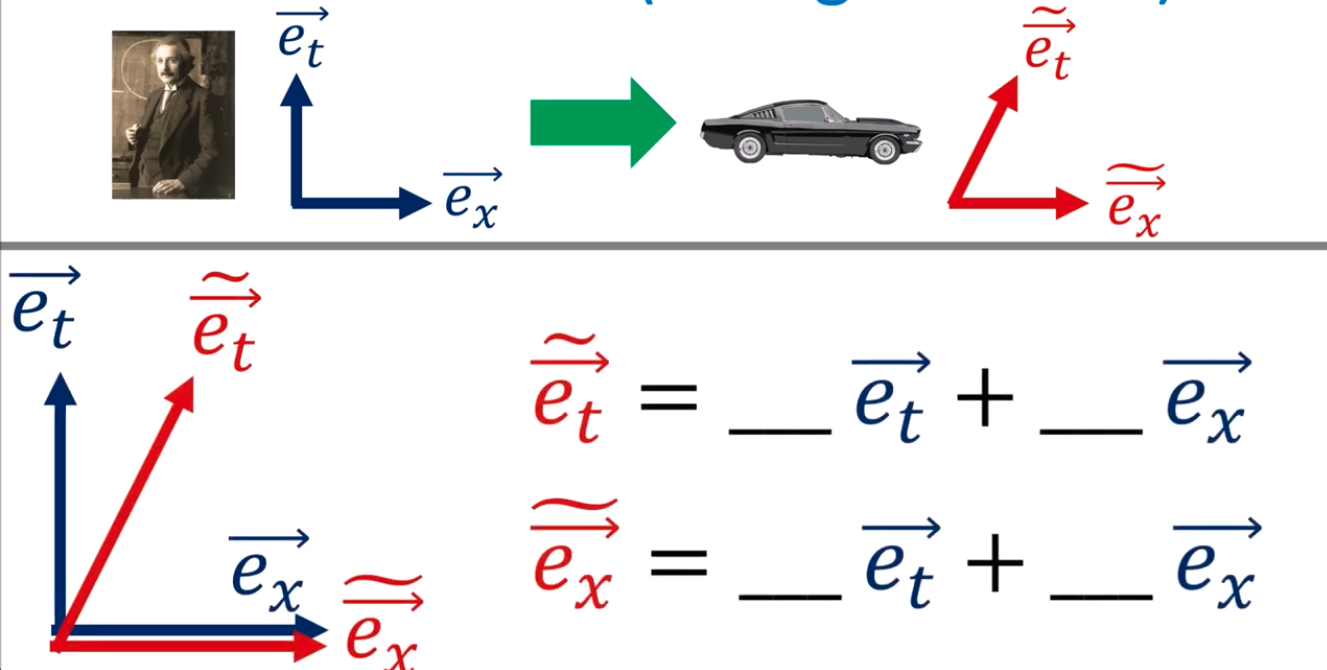
\includegraphics[scale=0.2]{figures/gelilean-basis-change-01.png}
\end{center}

Just visualizing it, we can write down that:

\begin{align*}
    \begingroup\color{red}\tilde{\vec{e}}_t\endgroup &= 1 \begingroup\color{blue}\vec{e}_t\endgroup + 1/2 \begingroup\color{blue}\vec{e}_x\endgroup = \begingroup\color{blue}\vec{e}_t\endgroup + 1/2 \begingroup\color{blue}\vec{e}_x\endgroup\\
    \begingroup\color{red}\tilde{\vec{e}}_x\endgroup &= 0 \begingroup\color{blue}\vec{e}_t\endgroup + 1 \begingroup\color{blue}\vec{e}_x\endgroup = \begingroup\color{blue}\vec{e}_x\endgroup
\end{align*}

In the other direction, we can also write down:

\begin{align*}
    \begingroup\color{blue}\vec{e}_t\endgroup &= \begingroup\color{red}\tilde{\vec{e}}_t\endgroup - 1/2 \begingroup\color{red}\tilde{\vec{e}}_x\endgroup\\
    \begingroup\color{blue}\vec{e}_x\endgroup &= \begingroup\color{red}\tilde{\vec{e}}_x\endgroup
\end{align*}

So now we have equations to move from one basis (scientist frame) to the other (car frame).
In terms of math, we can also prove easily that, one trasformation is the opposite to the other.\\

To prove that this is also valid generically, we can substitute the $1/2$ with the constant velocity the car's going $v$, both for the basis vectors and the 
components, to find out that we can write:\\ \\

\textbf{Basis: Man $\to$ Car}
\begin{align*}
    \begingroup\color{red}\tilde{\vec{e}}_t\endgroup &= \begingroup\color{blue}\vec{e}_t\endgroup + \begingroup\color{teal}v\endgroup \begingroup\color{blue}\vec{e}_x\endgroup \\
    \begingroup\color{red}\tilde{\vec{e}}_x\endgroup &= \begingroup\color{blue}\vec{e}_x\endgroup
\end{align*}

\textbf{Basis: Car $\to$ Man}
\begin{align*}
    \begingroup\color{blue}\vec{e}_t\endgroup &= \begingroup\color{red}\tilde{\vec{e}}_t\endgroup - \begingroup\color{teal}v\endgroup \begingroup\color{red}\tilde{\vec{e}}_x\endgroup\\
    \begingroup\color{blue}\vec{e}_x\endgroup &= \begingroup\color{red}\tilde{\vec{e}}_x\endgroup
\end{align*}

\textbf{Components: Man $\to$ Car}
\begin{align*}
    \begingroup\color{red}\tilde{t}\endgroup &= \begingroup\color{blue}t\endgroup\\
    \begingroup\color{red}\tilde{x}\endgroup &= -\begingroup\color{teal}v\endgroup \begingroup\color{blue}t\endgroup + \begingroup\color{blue}x\endgroup
\end{align*}

\textbf{Components: Car $\to$ Man}
\begin{align*}
    \begingroup\color{blue}t\endgroup &= \begingroup\color{red}\tilde{t}\endgroup\\
    \begingroup\color{blue}x\endgroup &= \begingroup\color{teal}v\endgroup \begingroup\color{red}\tilde{t}\endgroup + \begingroup\color{red}\tilde{x}\endgroup 
\end{align*}

The Galilean transform are basically all these formulas put together.\\
All of it becomes much easier if we write these down in matrix/array notation. 
Starting with the basis vector change from Man to Car, we can write down those in this form:

\begin{align*}
    \begin{bmatrix}
        \begingroup\color{red}\tilde{\vec{e}}_t\endgroup & \begingroup\color{red}\tilde{\vec{e}}_x\endgroup
    \end{bmatrix} &= 
    \begin{bmatrix}
        \begingroup\color{blue}\vec{e}_t\endgroup & \begingroup\color{blue}\vec{e}_x\endgroup
    \end{bmatrix}
    \begin{bmatrix}
        1 & 0\\
        \begingroup\color{teal}v\endgroup & 1
    \end{bmatrix}
\end{align*}

The components from Man to Car:
 
\begin{align*}
    \begin{bmatrix}
        \begingroup\color{red}\tilde{t}\endgroup\\ 
        \begingroup\color{red}\tilde{x}\endgroup
    \end{bmatrix} &= 
     \begin{bmatrix}
        1 & 0\\
        -\begingroup\color{teal}v\endgroup & 1
    \end{bmatrix}
    \begin{bmatrix}
        \begingroup\color{blue}t\endgroup\\ 
        \begingroup\color{blue}x\endgroup
    \end{bmatrix}
\end{align*}

The two Galilean matrixes are inverse of each other, you can easily prove that by multiplying by each other and obtaining the Identity matrix.\\
And then, you can easily prove yourself that, the Galilean matrix used to bring the basis vectors from Man to Car is the one to use
to bring the components from the Car to Man, and that the other Galilean matrix used to bring the basis vectors from Car to Man, is the one to use
to bring the components from Man to Car. If you read this carefully, you will then understand the reason of calling basis vectors covariant, and 
components contravariant.\\
Change-of-basis equation and Change-of-component equation use inverse Galilean matrices because of covariance and contravariance.\\

When writing in matrix/array form, remember to write the covariant basis vectors as rows, and place them on the left of matrix equation, 
and components (contravariant) vectors as column, on the right of the matrix multiplication. This in order to have the correct formulaes coming out of them.

\subsection{Metric Tensor}

The metric tensor concept, in the spacetime diagrams of Galilean relativity do not make much sense, so 
we'll discuss briefly this concept using the 2D flat plane. Briefly because this has been covered very well
in the Tensor for Beginners and Tensor Calculus lecture notes.\\

The metric tensor answers the question on how do we properly measure lengths in space.
If you simply plot a vector on the 2D plane, you can straight forward think that, by decomponsing it 
as linear combination of the two basis vectors, you can apply Pythagora's theorem and call it a day.\\
Unfortunately this does not work consistently, and only works out the real vector length when using orthonormal basis vectors (i.e. 
perpendicular basis vectors with units of 1).
If you try computing the length of a vector in different non-orthonormal basis, you end up with different answers.\\

The proper way of calculating the length is by using the dot product of the vector with itself. This works regardless
of the basis vectors/reference frame utilized.\\

\begin{equation}
    \|\begingroup\color{violet}\vec{R}\endgroup \|^2 =  \begingroup\color{violet}\vec{R}\endgroup \cdot \begingroup\color{violet}\vec{R}\endgroup
\end{equation}

If you write the vector as linear combination of the basis vectors you use, for example in 2D flat plane:

\begin{align*}
    \|\begingroup\color{violet}\vec{R}\endgroup \|^2 &=  \begingroup\color{violet}\vec{R}\endgroup \cdot \begingroup\color{violet}\vec{R}\endgroup\\
    &= \left(\begingroup\color{cyan}x\endgroup\begingroup\color{blue}\vec{e_x}\endgroup + \begingroup\color{cyan}y\endgroup\begingroup\color{blue}\vec{e_y}\endgroup\right) \cdot
    \left(\begingroup\color{cyan}x\endgroup\begingroup\color{blue}\vec{e_x}\endgroup + \begingroup\color{cyan}y\endgroup\begingroup\color{blue}\vec{e_y}\endgroup\right)\\
    &= \begingroup\color{cyan}xx\endgroup\left(\begingroup\color{blue}\vec{e_x}\endgroup \cdot \begingroup\color{blue}\vec{e_x}\endgroup\right) 
    + \begingroup\color{cyan}xy\endgroup\left(\begingroup\color{blue}\vec{e_x}\endgroup \cdot \begingroup\color{blue}\vec{e_y}\endgroup\right) 
    + \begingroup\color{cyan}yx\endgroup\left(\begingroup\color{blue}\vec{e_y}\endgroup \cdot \begingroup\color{blue}\vec{e_x}\endgroup\right) 
    + \begingroup\color{cyan}yy\endgroup\left(\begingroup\color{blue}\vec{e_y}\endgroup \cdot \begingroup\color{blue}\vec{e_y}\endgroup\right)\\
    &= \begin{bmatrix}
        \begingroup\color{cyan}x\endgroup&
        \begingroup\color{cyan}y\endgroup
    \end{bmatrix}
    \begin{bmatrix}
        \begingroup\color{blue}\vec{e_x}\endgroup \cdot \begingroup\color{blue}\vec{e_x}\endgroup & \begingroup\color{blue}\vec{e_x}\endgroup \cdot \begingroup\color{blue}\vec{e_y}\endgroup\\
        \begingroup\color{blue}\vec{e_y}\endgroup \cdot \begingroup\color{blue}\vec{e_x}\endgroup & \begingroup\color{blue}\vec{e_y}\endgroup \cdot \begingroup\color{blue}\vec{e_y}\endgroup
    \end{bmatrix}
    \begin{bmatrix}
        \begingroup\color{cyan}x\endgroup\\
        \begingroup\color{cyan}y\endgroup
    \end{bmatrix}\\
    &= \begin{bmatrix}
        \begingroup\color{cyan}x\endgroup&
        \begingroup\color{cyan}y\endgroup
    \end{bmatrix}
    \begin{bmatrix}
        \begingroup\color{blue}g_{xx}\endgroup & \begingroup\color{blue}g_{xy}\endgroup \\
        \begingroup\color{blue}g_{yx}\endgroup & \begingroup\color{blue}g_{yy}\endgroup  
    \end{bmatrix}
    \begin{bmatrix}
        \begingroup\color{cyan}x\endgroup\\
        \begingroup\color{cyan}y\endgroup
    \end{bmatrix}
\end{align*}

where that matrix is the representation of the metric tensor, and its components are basically the 
dot products of the basis vectors.\\

Trying to tie up everything together with the concept of invariance, we can say that, the length (or length squared) of a vector 
$\color{violet}\vec{R}$ has different formulas when computed in different reference frames, but the results are always equal and invariant 
as long as we use the metric tensor components related to the specific basis.\\

The metric tensor itself is a function, which takes two vectors as input, and spits out their dot product as output.
The output does not depend on the specific coordinate systems, which means that \textbf{the metric tensor itself is an invariant.}
It will just have different numbers/components in different coordinate systems, but so will the vector components of the two input vectors.\\

Worth noticing what happens to the metric tensor in terms of covariance/contravariance, so like, 
whay happens to the components of the metric tensor when we shrink/grow/rotate the basis vectors from one set to another?
It can be easily seen that, the metric tensor is 2-covariant, which means that when the basis vectors change, the metric tensor
changes in the same way, twice.

\subsection{Problems of Galilean Relativity}

So to recap, in Galilean Relativity, time is absolute and observers in differente reference frames will indeed agree on time, but will disagree on position.
We can convert between different reference frames using Galilean transform equations, for example between a man and a car reference frames:

\begin{align*}
    \begingroup\color{red}\tilde{t}_{car}\endgroup &= \begingroup\color{blue}t_{man}\endgroup = t\\
    \begingroup\color{red}\tilde{x}_{car}\endgroup &= \begingroup\color{blue}x_{man}\endgroup - \begingroup\color{teal}v\endgroup \begingroup\color{blue}t_{man}\endgroup
\end{align*}

From these, we can easily find the velocities convertion by differentiating with respect to time:

\begin{align*}
    \frac{d \begingroup\color{red}\tilde{x}_{car}\endgroup}{dt} = \frac{d \begingroup\color{blue}x_{man}\endgroup}{dt} - \begingroup\color{teal}v\endgroup
\end{align*}

This gives us the momentum transformation formula for free:

\begin{align*}
    \begingroup\color{blue}p_{man}\endgroup &= m \frac{d \begingroup\color{blue}x_{man}\endgroup}{dt}\\
    \begingroup\color{red}\tilde{p}_{car}\endgroup &= m \frac{d \begingroup\color{red}\tilde{x}_{car}\endgroup}{dt}
\end{align*}

And kinetic Energy:

\begin{align*}
    \begingroup\color{blue}E_{man}\endgroup &= \frac{1}{2} m \left(\frac{d \begingroup\color{blue}x_{man}\endgroup}{dt}\right)^2\\
    \begingroup\color{red}\tilde{E}_{car}\endgroup &= \frac{1}{2} m \left(\frac{d \begingroup\color{red}\tilde{x}_{car}\endgroup}{dt}\right)^2
\end{align*}

So, the most difficult thing to do in Gelilean Relativity, is calculating the position in different reference frames, and from there, calculating 
velocity, momentum and kinetic energy is very easy.\\

But what about the things we agree on? We know we agree on the laws of motion in different reference frames, like Newton's second law, and Newton's law of gravity. They both should
be invariant in different inertial reference frames.\\

We can easily see that if we try to compute the Newton's second law of motion, considering a shift in position (which is indeed what changes between observers in Galilean relativity):

\begin{align*}
    F = m \frac{d^2}{dt^2}\left[\begingroup\color{blue}x\endgroup(t) + \begingroup\color{violet}k\endgroup\right] = m \frac{d^2 \begingroup\color{blue}x\endgroup(t)}{dt^2} + m \cancel{\frac{d^2 \begingroup\color{violet}k\endgroup(t)}{dt^2}} = m \frac{d^2 \begingroup\color{blue}x\endgroup(t)}{dt^2}
\end{align*}

The derivative of the shift in position goes to zero, as it's not dependent on time. Similar can be seen for a reference frame moving at constant speed with respect to another one, so:

\begin{align*}
    F = m \frac{d^2}{dt^2}\left[\begingroup\color{blue}x\endgroup(t) + \begingroup\color{teal}v\endgroup t\right] = m \frac{d^2 \begingroup\color{blue}x\endgroup(t)}{dt^2} + m \frac{d^2}{dt^2}(\begingroup\color{teal}v\endgroup t) = m \frac{d^2 \begingroup\color{blue}x\endgroup(t)}{dt^2} + m \cancel{\frac{d}{dt}(\begingroup\color{teal}v\endgroup)} = m \frac{d^2 \begingroup\color{blue}x\endgroup(t)}{dt^2}
\end{align*}

So even in this case, we've shown that a constant speed shift in position does not alter the law of motion.\\

Now let's try adding a second order term to the position, which is like changing coordinates to an accelerated reference frame:

\begin{align*}
    F = m \frac{d^2}{dt^2}\left[\begingroup\color{blue}x\endgroup(t) + \frac{1}{2}\begingroup\color{red}\alpha\endgroup t^2\right] = m \frac{d^2 \begingroup\color{blue}x\endgroup(t)}{dt^2} + m \frac{d^2}{dt^2}\left(\frac{1}{2}\begingroup\color{red}\alpha\endgroup t^2\right) = m \frac{d^2 \begingroup\color{blue}x\endgroup(t)}{dt^2} + m \begingroup\color{red}\alpha\endgroup
\end{align*}

So this shows that in accelerating reference frame, Newton's second law does not hold true, as we end up with an extra term due to the fictitious force. This fictitious force is why 
you feel your body pulled downward in an elevator that's accelerating upward, or thrown back into the seat in a car accelerating forward.\\

Now what about Electromagnetism laws? Are they invariant under Galilean transform? In other words, is the force vector due to electricity and magnetism (aka Lorentz Force)
the same in all inertial reference frames?

\begin{equation}
    \vec{F} = q\begingroup\color{blue}\vec{E}\endgroup + q\left(\begingroup\color{blue}\vec{v}\endgroup \times \begingroup\color{blue}\vec{B}\endgroup\right) = q\begingroup\color{red}\tilde{\vec{E}}\endgroup + q\left(\begingroup\color{red}\tilde{\vec{v}}\endgroup \times \begingroup\color{red}\tilde{\vec{B}}\endgroup\right)
\end{equation}

Well the short answer is no, laws of electromagnetism are not invariant under the Galilean transform, and the ultimate reason for this is that the speed of light is 
invariant in all reference frames, which leads to special relativity. Which fixes the first of these problems.\\

The proof can be seen with an example experiment of a moving charge, where you have an electric wire with current going through, and you examine what a moving charge 
outside of the wire will experience. In the lab reference frame, the charge outside is moving with respect to the wire, and will experience a magnetic field resulting from the current density
along the wire. As a result, the charge will experience a force due to the magnetic field.\\
In the charge's rest frame, its velocity is stationary, and by Galilean relativity, there's no relative motion, so the observer concludes that the magnetic 
force is zero, and they only observe a static electric field and the corresponding electrostatic force.\\

The contradiction is solved by using Lorents transformation, which incorporates the constancy of the speed of light, length contraction, and time dilation. Because distances and time intervals change between moving reference frames, the charge density and electric/magnetic fields are also transformed. 
This reveals that electric and magnetic fields are two sides of the same coin (the electromagnetic field).\\
By using the Lorentz Transformation, both observers will calculate the exact same net physical force on the particle, even if one describes it as entirely magnetic and the other describes it as entirely electric.\\

Furthermore, we can easily show by manipulating the Maxwell's equations, that the resulting Wave equations (Helmholtz Equations), clearly show the constant speed of light.\\

Considering the Maxwell's Equations with no sources ($\rho = 0$, $\vec{J} = 0$), and using a vector identity for which the rotor of a the rotor is equal to the gradient of the divergence minus
the laplacian, we obtain the electric and magnetic wave equations:

\begin{align*}
\nabla^2\vec{E} &= \begingroup\color{teal}\mu_0\endgroup \begingroup\color{brown}\epsilon_0\endgroup \frac{\partial^2 \vec{E}}{\partial t^2}\\
\nabla^2\vec{B} &= \begingroup\color{teal}\mu_0\endgroup \begingroup\color{brown}\epsilon_0\endgroup \frac{\partial^2 \vec{B}}{\partial t^2}
\end{align*}

Knowing that in wave equations like these, the speed of the wave is given by the inverse of the coefficient multiplying the second-order time derivative, under square root:

\begin{equation}
    c = \frac{1}{\sqrt{\begingroup\color{teal}\mu_0\endgroup \begingroup\color{brown}\epsilon_0\endgroup}}
\end{equation}

These two numbers are respectively ($\begingroup\color{teal}\mu_0\endgroup$), the magnetic permeability of the vacuum, and ($\begingroup\color{brown}\epsilon_0\endgroup$)
the electric permittivity of the vacuum. Both are well known physical constants, and if you plug them in, you will find out that the speed of an electromagnetic wave is equal 
to the well know value:

\begin{equation}
    c = \frac{1}{\sqrt{\begingroup\color{teal}\mu_0\endgroup \begingroup\color{brown}\epsilon_0\endgroup}} = 
    \frac{1}{\sqrt{(8.854 \times 10^{-12})(1.257 \times 10^{-6})}} = 2.998 \times 10^{8} m/s
\end{equation}

This is strong theoretical evidence that the speed of light is a law of physics itself, and the same in all reference frames. Of course, theory does not mean anything
unless it agreed with physical experimental evidence.\\

Physicists have tried in the past, in the late 1800, to validate that their theory that light travels in a special reference frame, absolutely stationary, called ether.\\
The famous Michelson-Morley experiment had shown no difference in the speed of light in perpendicular directions, which provided strong experimental evidence that there's no special absolute frame of reference, 
and that the speed of light is constant in all inertial reference frames.\\

This led to Einstein's postulates of Special Relativity, that we'll study in the next section.
We'll see how different inertial reference frames disagree on time (time dilation) and lenghts (length contraction), as well as 
how to take derivative with respect to time (i.e. velocity), we'll also see that we cannot simply add velocities together, as the speed of light $c$ is constant, 
and the laws of motion will require some re-thinking to be maintained the same between inertial reference frames.\\

